\documentclass[12pt, a4paper]{article}
% Packages to use:
\usepackage{afterpage}
\usepackage{algorithm}
\usepackage{algorithmicx}
\usepackage{algpseudocode}
%\usepackage{apacite} % Didn't work
\usepackage{authblk}
\usepackage{amsmath}
\usepackage[title]{appendix}
\usepackage{amsfonts}
\usepackage{booktabs} % For \toprule, \midrule, \botrule
\usepackage[citestyle = apa, bibstyle=apa, maxbibnames=20]{biblatex}
\usepackage[font=small,labelfont=bf, hypcap=false]{caption} %\caption
\usepackage{chngcntr}
\usepackage{comment} %large comment
\usepackage{csquotes} % Include csquotes
\usepackage{csvsimple} % CSV to latex
\usepackage{diagbox}
\usepackage{enumitem}
\usepackage{eqnarray}
\usepackage{float} % for customizing caption position
\usepackage[T1]{fontenc} % Font encoding
\usepackage{geometry}
\usepackage{graphicx}
\usepackage[colorlinks=true, allcolors=blue]{hyperref}
\usepackage[none]{hyphenat} % Hyphonate
\usepackage{lineno} % Add the lineno package
\usepackage{listings}
\usepackage{lipsum}
\usepackage{longtable}
\usepackage{lscape}
\usepackage{mathrsfs}
\usepackage{multirow}
\usepackage{orcidlink}
\usepackage{pdflscape}
\usepackage[]{ragged2e}
\usepackage{subcaption}
\usepackage{setspace} % Customize line spacing
\usepackage{threeparttable} %For table footnotes
\usepackage{tabularray}
\usepackage{titlesec} % Redefine (sub)section numbering

% ---- References & citations ---
% Your reference file:
\addbibresource{refs.bib} % Your.bib file
%\bibliographystyle{apa}

% Set page size and margins
\geometry{a4paper,
        top=1in,
        bottom=1in,
        left=1in,
        right=1in,
        marginparwidth=0.5in
        }
        
\onehalfspacing % 1.5 line spacing
\titleformat{\section} % Redefine section numbering format
{\normalfont\Large\bfseries}{\thesection.}{1em}{}

% Line Numbering:
\renewcommand\linenumberfont{\normalfont\scriptsize\sffamily\color{blue}}
\linenumbers % Enable line numbering
\rightlinenumbers % Right-align; comment this line for left alignment.

% Define a new command for the fourth-level title.
\newcommand{\subsubsubsection}[1]{%
  \vspace{\baselineskip} % Add some space
  \noindent\textbf{#1\\}\quad % Adjust formatting as needed
}

% Change the position of the table caption above the table
\captionsetup[table]{position=top} % caption position for tables

% Define the unnumbered list
\makeatletter
\newenvironment{unlist}{%
  \begin{list}{}{%
    \setlength{\labelwidth}{0pt}%
    \setlength{\labelsep}{0pt}%
    \setlength{\leftmargin}{2em}%
    \setlength{\itemindent}{-2em}%
    \setlength{\topsep}{\medskipamount}%
    \setlength{\itemsep}{3pt}%
  }%
}{%
  \end{list}%
}
\makeatother
% Suppress the warning about \@parboxrestore
%\pdfsuppresswarningpagegroup=1

%-------------------------------------------
% Paper Head
%-------------------------------------------
\title{\textbf{Title Here}}
\author[1, 2, *]{\small FirstName MiddleName LastName \orcidlink{xxxx-xxxx-xxxx-xxxx}}
\author[2]{\small FirstName MiddleName LastName}
\author[3]{\small FirstName MiddleName LastName \orcidlink{xxxx-xxxx-xxxx-xxxx}}
\affil[1]{\small{Name of the Department, Organization, City, State, Zip Code}}
\affil[2]{\small{Name of the Department, Organization, City, State, Zip Code}}
\affil[3]{\small{Name of the Department, Organization, City, State, Zip Code}}
\affil[*]{Corresponding author: \href{mailto:email@mail.com}{email@mail.com}; \href{mailto:email@mail.edu}{email@mail.edu}}
\date{}

\begin{document}
\newpage
\maketitle
\begin{abstract}
{Abstract here}
\end{abstract}

\noindent\textbf{Keywords}: 5-6 Keywords \\
\noindent\textbf{JEL Codes}: For economics articles only \hspace*{\fill}

\newpage
%-------------------------------------------
% Paper Body
%-------------------------------------------
\newpage
\section*{Highlights}
\begin{itemize}
    \item Problem and solution
    \item Method
    \item Result 1 / Recommendations / Policy Implications
    \item Result 2 / Recommendations / Policy Implications
    \item Result 3 / Recommendations / Policy Implications / Conclusion
\end{itemize}

\newpage
\section{Introduction}

\begin{center}
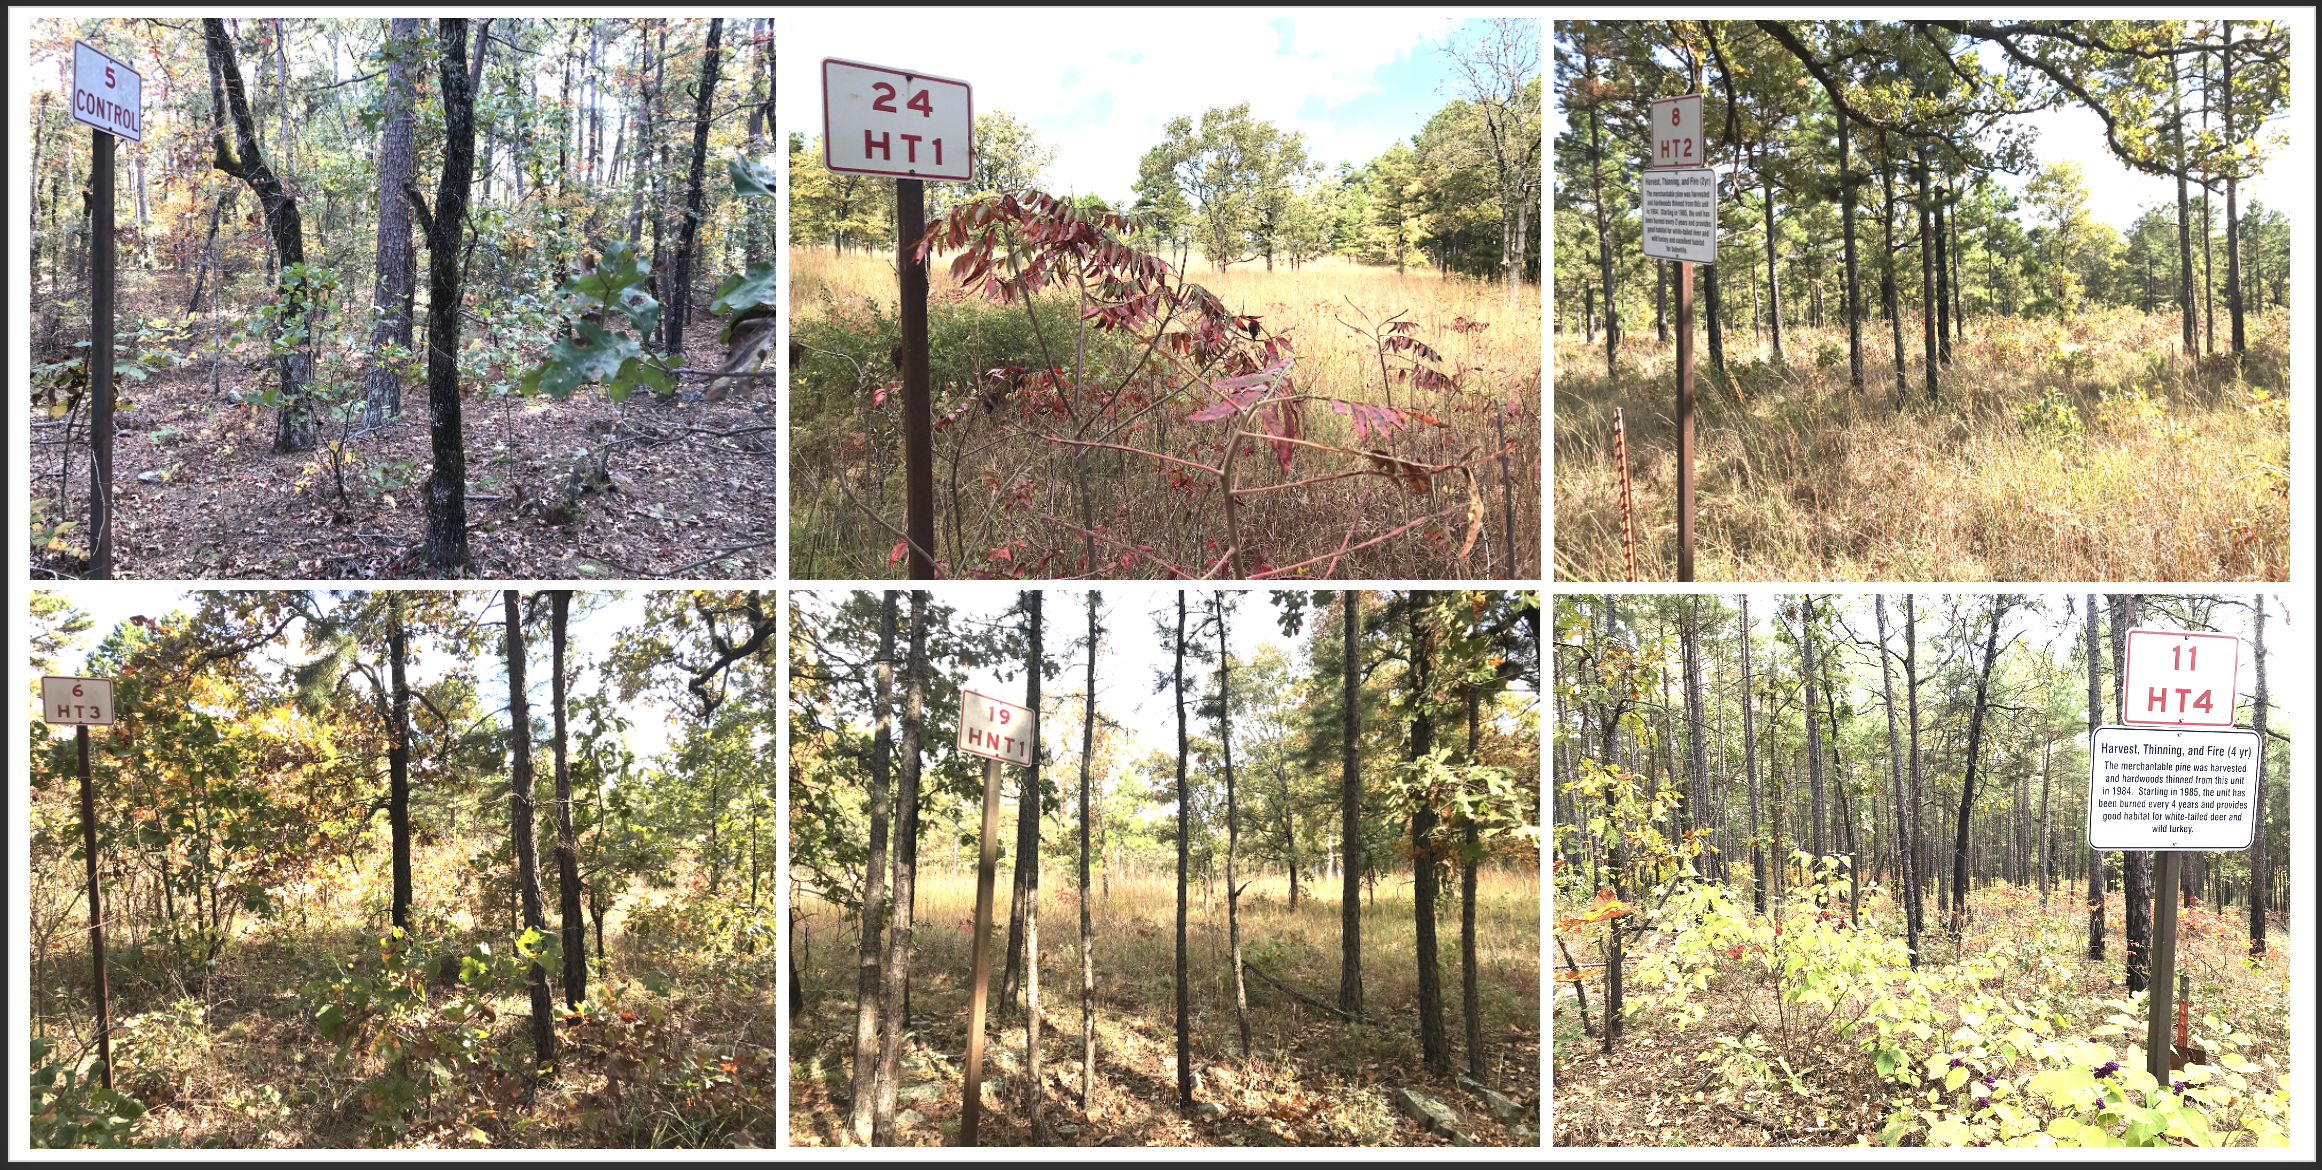
\includegraphics[scale = 0.39, trim ={0.2cm, 0.2cm, 0.2cm, 0.2cm}, clip] {figures/Push.png}
\captionof{figure}{\small Caption of figure}
\label{Figure: Push}
\end{center}

\begin{itemize}
    \item \verb|\parencite[]{yang2024soil}|  gives \parencite[]{yang2024soil} 
    \item \verb|\enquote{\$6 fee}| gives \enquote{\$6 fee}
    \item \verb|\cite{yang2024soil}| gives \cite{yang2024soil}
    \item \verb|\ref{tab:Demog}| gives \ref{tab:Demog}
    \item \verb|\ref{Figure: Push}| gives \ref{Figure: Push}
\end{itemize}

\section{Theoretical Foundation}

\section{Method}
\subsection{Subsection}

\noindent The probability of ... was estimated as
\begin{multline}\label{Prob}
P_{BW}(rr' = 1|\textbf{X}_{itk}) = \beta_{{CAN}}{{CAN}_{itk}} +  \\ \lambda_{{NSFP}}{{NSFP}_{itk}} +
\lambda_{{SFP}}{{SFP}_{itk}} + \epsilon_{{itk}}
\end{multline}
\noindent where the $\beta$s are ..., $\lambda$s are ..., and $\epsilon_{i}$ is stochastic error term.

\section{Results and Discussion}

\begin{longtable}[c]{rcccccc}
\caption{Demographics}
\label{tab:Demog} \\
\toprule
\multicolumn{1}{c}{\textbf{Demographic Variables}} & \textbf{N} & \textbf{Mean} & \textbf{Std. Dev.} & \textbf{Median} & \textbf{Min} & \textbf{Max} \\
\midrule
\multicolumn{1}{l}{Agricultural Cropland (Acres)}       & 134 & 196.47 & 513.36 & 80 & 0 & 5,500 \\
\multicolumn{1}{l}{Rangeland (Acres)}                   & 224 & 475.01 & 529.19 & 282.50 & 0 & 3,000 \\
\multicolumn{1}{l}{Forests (Acres)}                     & 200 & 209.56 & 417.49 & 100 & 0 & 3,500\\
\bottomrule
\multicolumn{7}{l}{\textbf{Notes:}}\\
\multicolumn{7}{l}{.....} \\
\end{longtable}

\begin{table*}[!ht]
\caption{Caption \label{Table: Labels}}
\tabcolsep=0pt
\begin{threeparttable}
\begin{tabular*}{\textwidth}{@{\extracolsep{\fill}}lccc@{\extracolsep{\fill}}}
\toprule
\multicolumn{1}{c}{Site }       & \multicolumn{1}{c}{Marginal(\$)}  & \multicolumn{1}{c}{$p > |z|$} & \multicolumn{1}{c}{95\% CI} \\
\multicolumn{1}{c}{Attributes}  & \multicolumn{1}{c}{(Std. Err.)}           &                               & \multicolumn{1}{c}{Lower, Upper} \\
\midrule
ABC & -0.96 (0.81) & 0.235 & -2.53, 0.62 \\
DEF & -0.71 (0.71) & 0.317 & -2.11, 0.69 \\
\bottomrule
\end{tabular*}
\begin{tablenotes}[para, flushleft]
\item Note: Marginal WTPs, Std. Err., and CIs were rounded to two decimal points. \\
\end{tablenotes}
\end{threeparttable}
\end{table*}

\newpage
\printbibliography

\newpage
%-------------------------------------------
% Appendix
%-------------------------------------------

\renewcommand\theequation{\Alph{section}\arabic{equation}} %Redefine equation numbering format
\counterwithin*{equation}{section} % Number equations within sections
\renewcommand\thefigure{\Alph{section}\arabic{figure}} % Redefine equation numbering format
\counterwithin*{figure}{section} % Number equations within sections
\renewcommand\thetable{\Alph{section}\arabic{table}} % Redefine equation numbering format
\counterwithin*{table}{section} % Number equations within sections

\newpage
\begin{appendices}

\section*{Appendix A: }

\section*{Appendix B:}

\end{appendices}
\end{document}